% указываем класс документа
\documentclass[12pt,a4paper,openany]{extarticle}

% подключаем собственный стилевой файл 
\usepackage{mystyle}

% указываем язык (для автоматической вставки слов, типа "Глава", "Содержание", "Литература", "рис." и пр.
\selectlanguage{russian}

\begin{document}
\part*{Лабораторная работа №3\\
 Управление двигателем постоянного тока}
\section{Методические рекомендации}
До начала работы студент должен выполнить предыдущие работы этого цикла. Необходимо знание основ теории автоматического управления.
\section{Теоретические сведения}
В~предыдущей лабораторной работе мы получили модель второго порядка для двигателя~NXT. 
\begin{equation}
W(s)=\frac{1/k_\omega}{T_eT_ms^2+T_ms+1}.
\end{equation}
Главной целью предыдущей было получение связи напряжения и угловой скорости. Для~задачи управления двигателем по~углу мы~можем воспользоваться моделью первого пордка. Если измерить индуктивность, она~действительно окажется достаточно маленькой, поэтому положим $L=0\Rightarrow T_e=0$:
\begin{equation}
W(s)=\frac{1/k_\omega}{T_ms+1}.
\end{equation}
Если нам необходимо получить на~выходе не скорость, а~угол, то мы должны проинтегрировать функцию оригинал, а в~образе Лапласа просто домножить на~$\cfrac1s$ (соответствующие математические выкладки можно найти в~книге «Интегральное преобразование и операционное исчисление» И.\,К.\,Волков):
\begin{equation}
W(s)=\frac{1/k_\omega}{s(T_ms+1)}.
\end{equation}
Теперь один из~корней равен 0, и график не сходится к нулю.

\begin{figure}[H]
	\noindent\centering{
		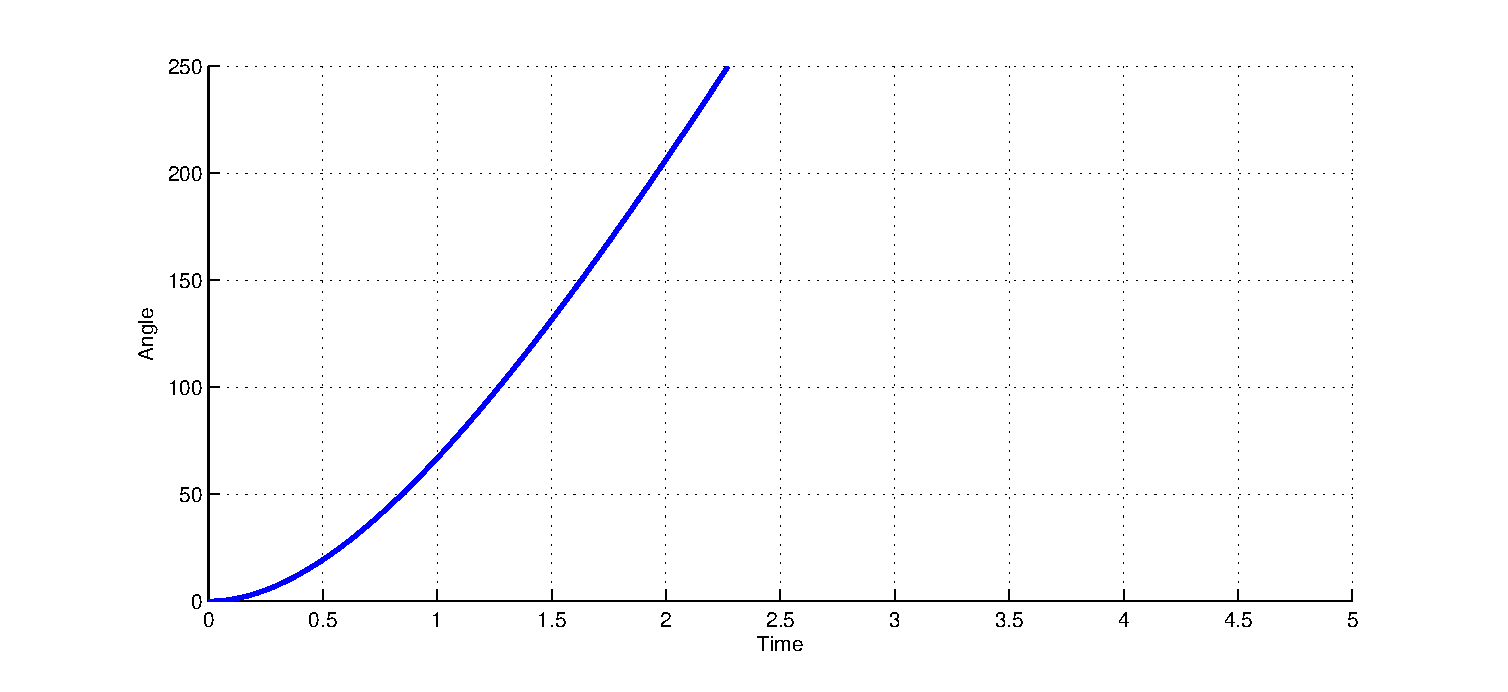
\includegraphics[scale=0.5]{1.eps}
	}
	\caption{Неустойчивая система.}
	\label{fig2}
\end{figure}					

Если подать на~двигатель постоянное напряжение, он~будет вращаться с постоянной скоростью, а~угол будет все~время увеличиваться.  Для того, чтобы стабилизировать значение угла, нам необходимо синтезировать регулятор (релейный, П, ПД или ПИД). Рассмотрим П"~регулятор. Для этого введем отрицательную обратную связь по~ошибке, умноженную на~пропорциональный коэффициент~K:

\begin{figure}[H]
	\noindent\centering{
		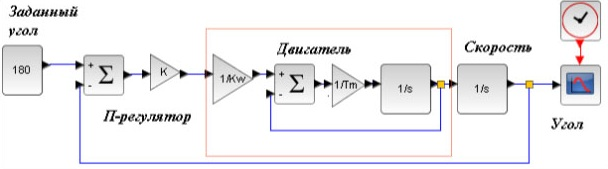
\includegraphics[scale=0.5]{2.jpg}
	}
	\caption{Система с отрицательной обратной связью.}
	\label{fig2}
\end{figure}

\begin{figure}[H]
	\noindent\centering{
		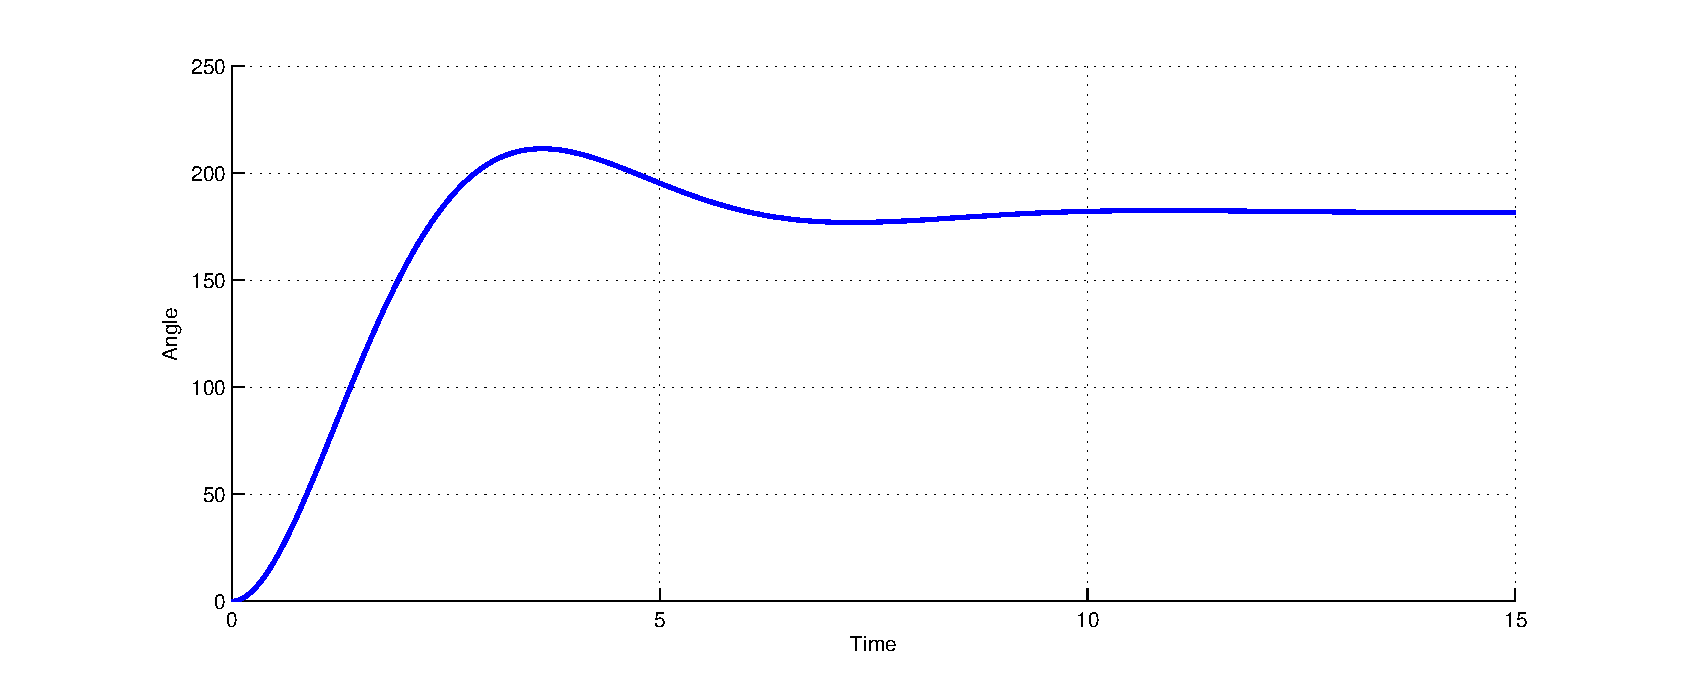
\includegraphics[scale=0.6]{3.eps}
	}
	\caption{График отработки заданного угла.}
	\label{fig3}
\end{figure}

Теперь получим передаточную функцию по ошибке:
\begin{equation}
W(s)=\frac{\cfrac{1/k_\omega}{s(T_ms+1)}}{1+\cfrac{1/k_\omega}{s(T_ms+1)}K}=\frac{1/k_\omega}{T_ms^2+s+K/k_\omega}.
\end{equation}
Найдем полюса функции: 
\begin{equation}
s_{1,2}=\frac{-1\pm\sqrt{1-4T_mK/k_\omega}}{2T_m}\Rightarrow -1\pm\sqrt{1-4T_mK/k_\omega}<0\Rightarrow -4T_mK/k_\omega <0.
\end{equation}
Следует вывод, для обеспечения устойчивости объекта с отрицательной обратной связью необходимо, чтобы коэффициент обратной связи был положительным. \\ 

\section{Цель работы}
Реализовать алгоритм отработки двигателем заданного угла. Получить показания угла двигателя при~различных значениях задержки.
\section{Порядок выполнения работы}
\begin{enumerate}
	\item Снятие показаний с двигателя NXT.
	\begin{enumerate}
		\item Соберите конструкцию так же как в первой работе.
		\item Реализуйте программу в~среде разработки, которая выполняет следующие действия: организует управление двигателем по~углу; снимает показания  угла поворота двигателя.
		\item Получите показания угла при~различных значениях интервала задержки и коэффициента обратной связи.
	\end{enumerate}
	\item Проверка расчетов.
	\begin{enumerate}
		\item Постройте схему полученной математической модели, используя Xcos.
		\item Осуществите моделирование системы.
		\item Сравните графики, полученные в~результате снятия экспериментальных данных и математического моделирования.
	\end{enumerate}
	\item Обработка данных.
	\begin{enumerate}
		\item Выведите графики экспериментальных значений вместе с~графиками моделирования.
	\end{enumerate}
\end{enumerate}
\section{Содержание отчета}
\begin{enumerate}
	\item Исходный код написанной программы.
	\item Полученные данные угла.
	\item Параметры математической модели.
	\item Переходная функция и уравнения математической модели двигателя NXT.
	\item Схема моделирования и график, полученные при~математическом моделировании.
\end{enumerate}
\end{document}